% Bismillahi-r-Rahmani-r-Rahim
\documentclass{article}
\author{Daoud Clarke}
\date{\today}
\title{Learning Lattice Orderings}

\usepackage{color}
\usepackage{graphicx}
\usepackage{amssymb}
\usepackage[round]{natbib}

\newtheorem{definition}{Definition}

\begin{document}

\maketitle

This document describes a method for learning a lattice ordering on a
vector space. The idea is based on the observation that a positive
cone can be described as an intersection of half-spaces, defined by a
plane passing through the origin.

The idea is to use multiple passes of a support vector machine to
learn multiple planes, which are used to define the cone.

\section{Experiment on a Toy Example}

We describe an experiment in two dimensions with 1000 points. A cone
is specified in this space, and points are classified according to
whether they are inside the cone. In the figures, points inside the
cone are shown as red circles, and other points as blue crosses.

\begin{figure}%
\begin{center}
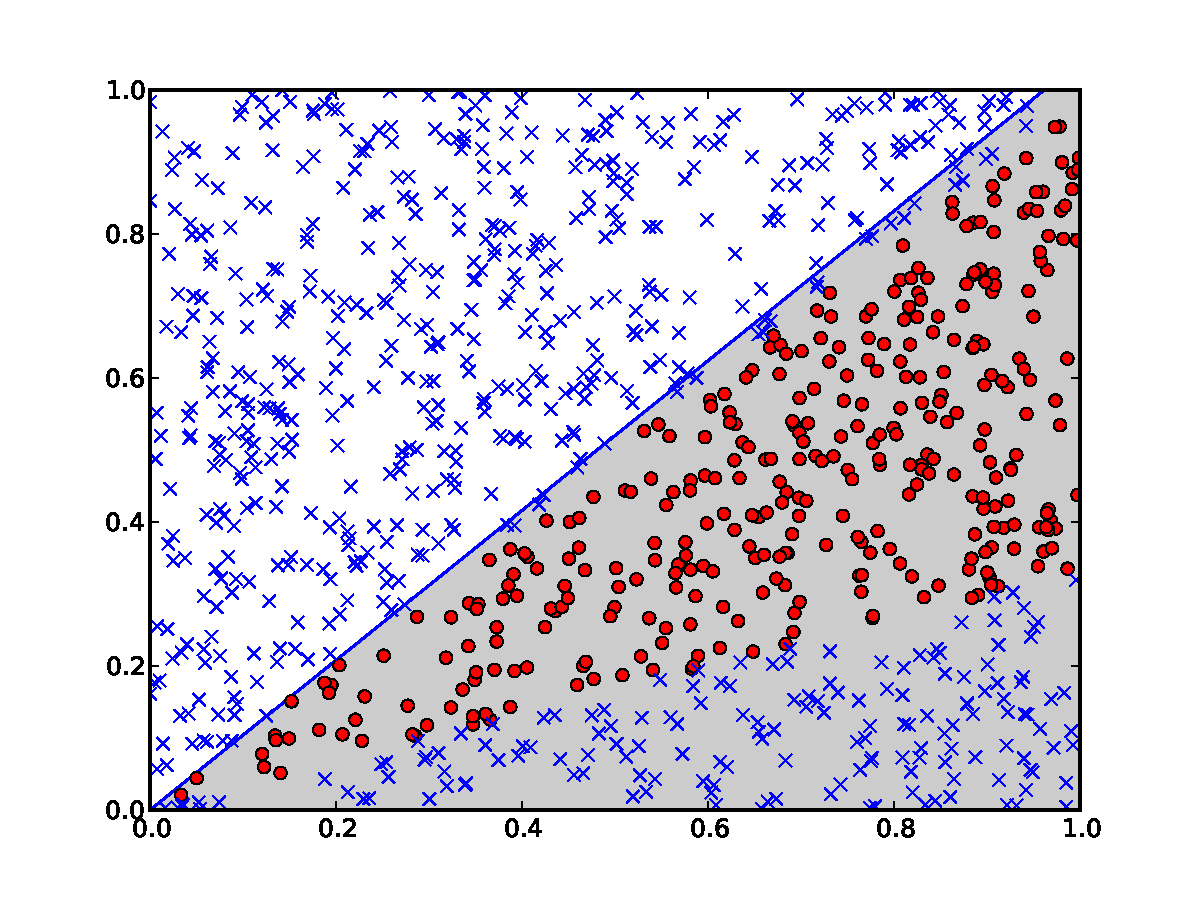
\includegraphics[scale=0.5]{first_plane.pdf}%
\caption{First plane learnt by the method}
\end{center}
\end{figure}%

Once a single plane has been learnt, any instances which are not
positive that are classified correctly are removed, and we perform a
second iteration, and so on, until we have $d$ planes, where $d$ is
the dimensionality of the space.

\begin{figure}%
\begin{center}
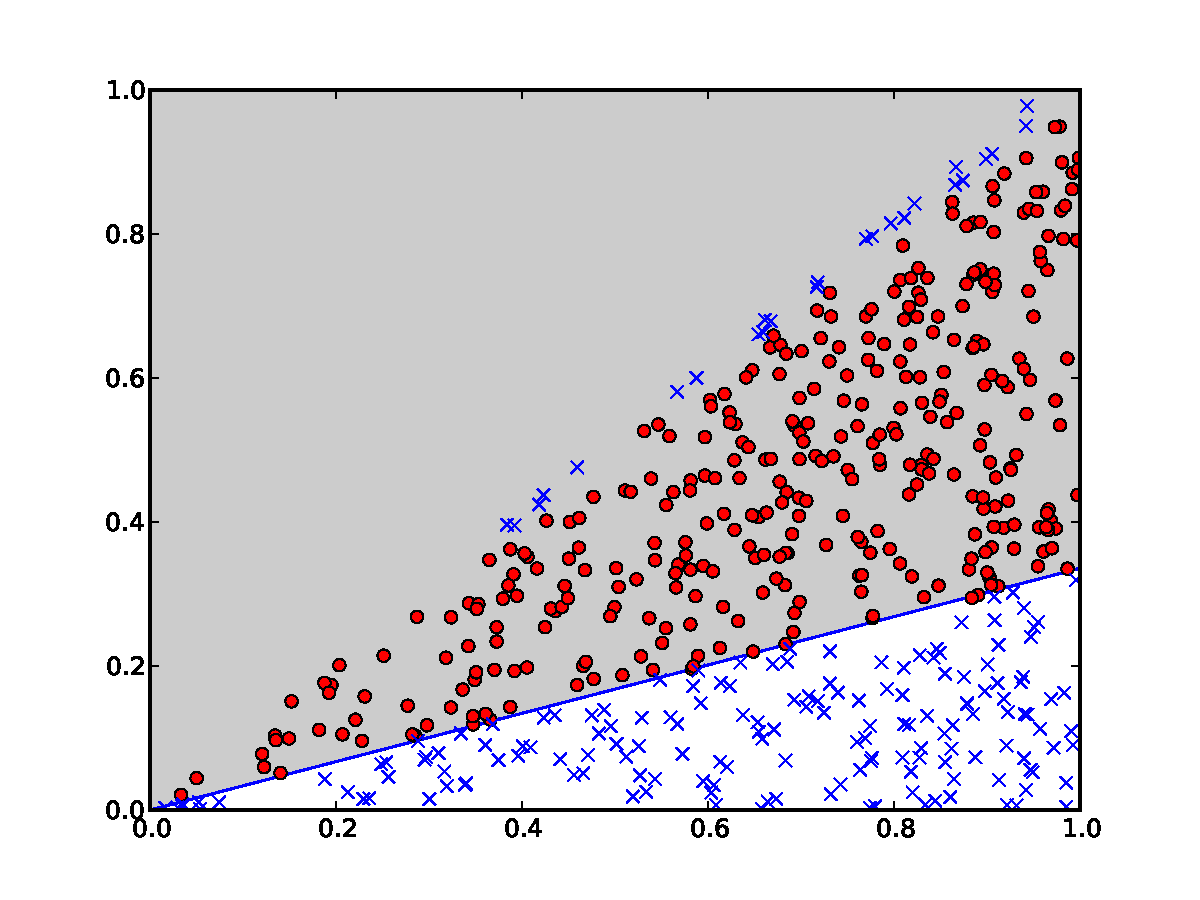
\includegraphics[scale=0.5]{second_plane.pdf}%
\caption{Second plane learnt by the method}
\end{center}
\end{figure}%

\subsection{Implementation Details}

Since we want our planes to pass through the origin, we need a support
vector machine implementation which allows us to specify that we want
\textbf{unbiased} planes. We use SVMLight, which allows this.

Since we wish to be able to learn with noisy data, we use a
soft-margin classifier. This means that the plane will not necessarily
cleanly separate the two classes, and it is sensitive to the cost
value specified for the SVM.

An important feature of our technique is that we have multiple passes
to identify points that are outside of the positive cone, therefore we
wish for high recall of the positive elements. Unfortunately, varying
the cost alone will not guarantee high recall because of the nature of
the data. In order to do this, we need to vary the cost of
misclassification per class. SVMLight allows us to do this by
specifying a cost-factor which determines the relative cost of
misclassification for the positive class.

We perform a grid search with cross validation, varying the cost and
the cost-factor. We use the F2 measure to evaluate points on the grid,
which allows us to emphasise the importance of recall of the positive
class.


\bibliographystyle{plainnat}

\bibliography{contexts}

\end{document}
